\doublespacing % Do not change - required

\chapter{DC Motor Matlab Modeling}

\thesisspacing % Do not change - required

Below you can see the modeling of a DC motor in the Simulink program and the internal structure of the DC motor.

\begin{figure}[H]
    \centering
    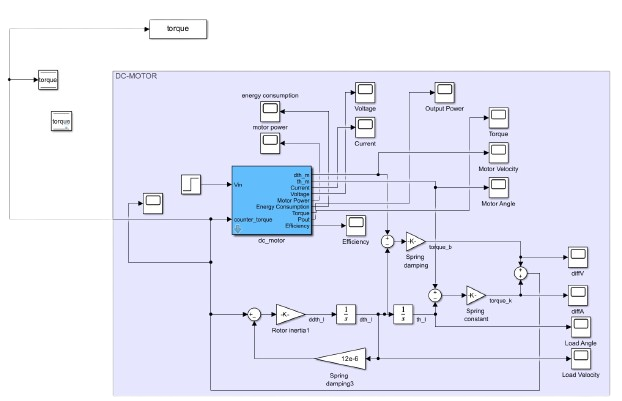
\includegraphics[width=0.9\columnwidth]{imgs/io/dc1.png}
    \caption[Simulink model of the DC motor]{Simulink model of the DC motor}
    \label{fig-magnitude}
\end{figure}%

A Simulink drawing of a DC model was created above. From here, the current, torque, etc. quantities were taken and the energy consumption and efficiency of the motor were measured.

\begin{figure}[h]
        \centering
        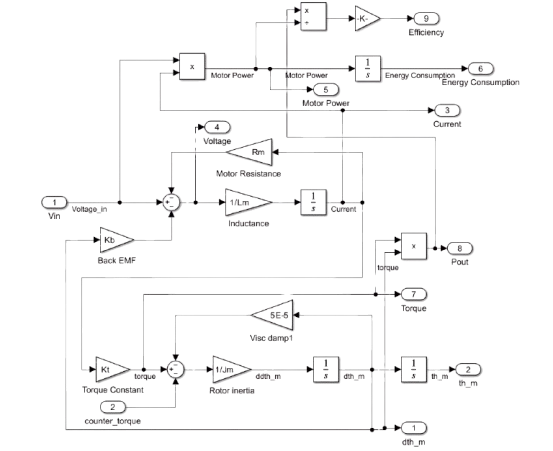
\includegraphics[width=0.9\columnwidth]{imgs/io/dc2.png}
        \caption[Inside of the DC motor]{Inside of the DC motor}
        \label{fig-magnitude}
\end{figure}%

The internal structure of a DC motor is shown above. Depending on these, any information desired from the current-time expression of the system to the efficiency expression can be obtained.

The current is equal to the integral of the output voltage divided by the inductance value with
respect to time. The current-time graph is shown below:


\begin{equation}
i = \int_{0}^{t} \frac{V_{\text{out}}}{L_m} \, dt 
\end{equation}



\begin{figure}[H]
    \centering
    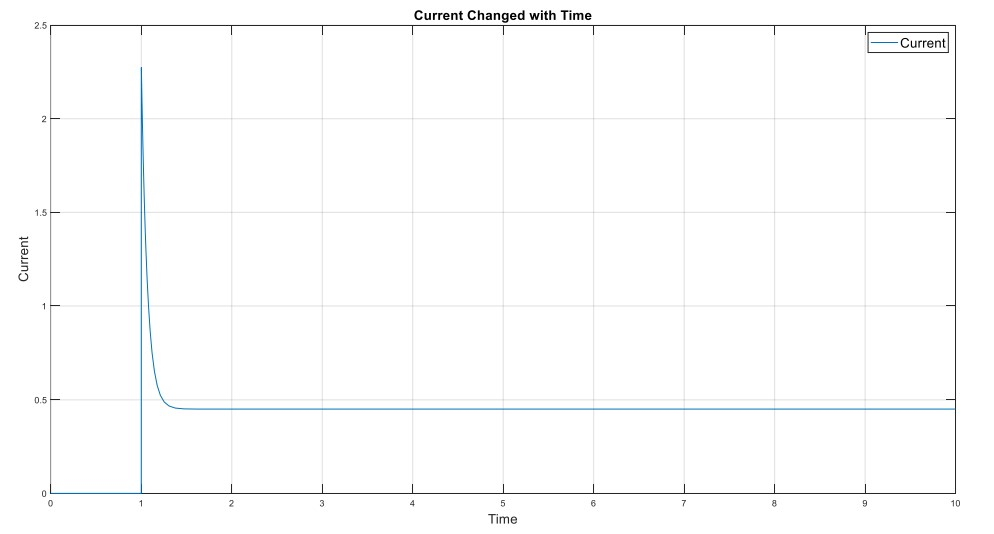
\includegraphics[width=0.7\columnwidth]{imgs/io/a.jpg}
    \caption[Current-time graph]{Current-time graph}
    \label{fig-magnitude}
\end{figure}%

Torque is equal to the product of the torque constant and the current. Below is the torque time
graph.

\begin{equation}
u = K_t i
\end{equation}

\begin{figure}[H]
    \centering
    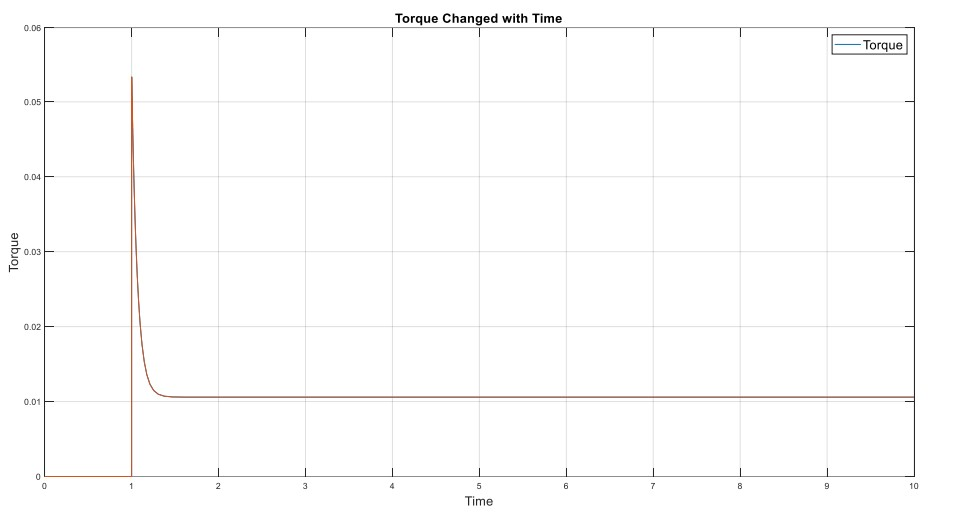
\includegraphics[width=0.7\columnwidth]{imgs/io/b.jpg}
    \caption[Torque-time graph]{Torque-time graph}
    \label{fig-magnitude}
\end{figure}%

The counter torque created by the load is as shown in the graph below. This acts as a
distorting effect on the DC motor.

\begin{figure}[H]
    \centering
    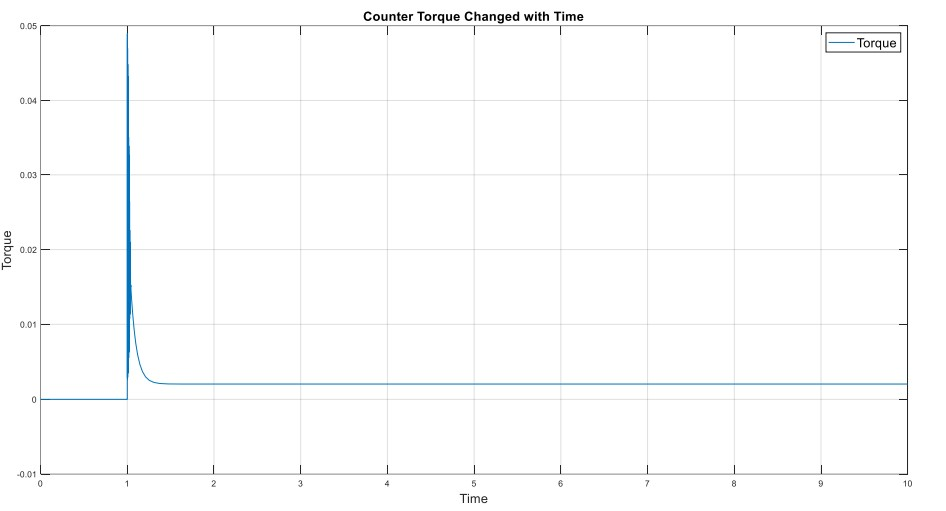
\includegraphics[width=0.7\columnwidth]{imgs/io/c.jpg}
    \caption[Counter torque-time graph]{Counter torque-time graph}
    \label{fig-magnitude}
\end{figure}%

The angular velocity of the motor is equal to the integral of the angular acceleration of the
motor. Here we see that the motor increases rapidly and then settles to a constant value.

\begin{equation}
w = \int_0^t \alpha \, dt    
\end{equation}

\begin{figure}[H]
    \centering
    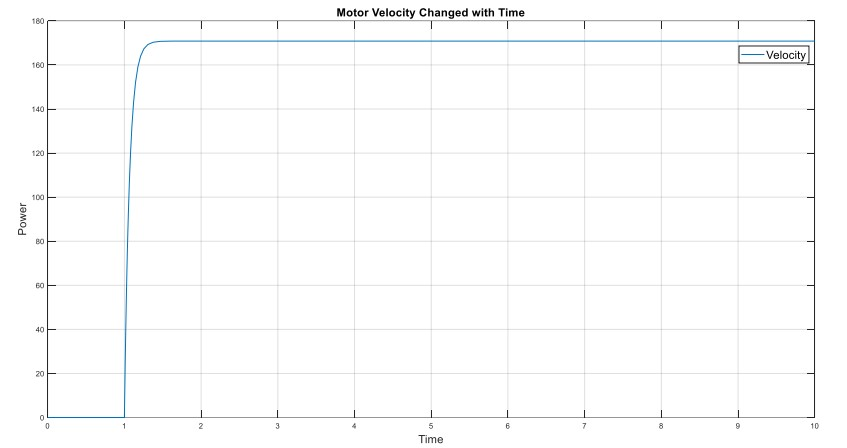
\includegraphics[width=0.7\columnwidth]{imgs/io/d.jpg}
    \caption[Angular velocity-time graph]{Angular velocity-time graph}
    \label{fig-magnitude}
\end{figure}%

The angular position of the motor, that is, its angle, is equal to the integral of the angular velocity
of the motor. In other words, it is the second integral of its angular acceleration. Here, it is seen
that the angular increases linearly. Its unit is radian.

\begin{equation}
\theta = \int_{0}^{t} \int_{0}^{t} \alpha \, dt    
\end{equation}

\begin{figure}[H]
    \centering
    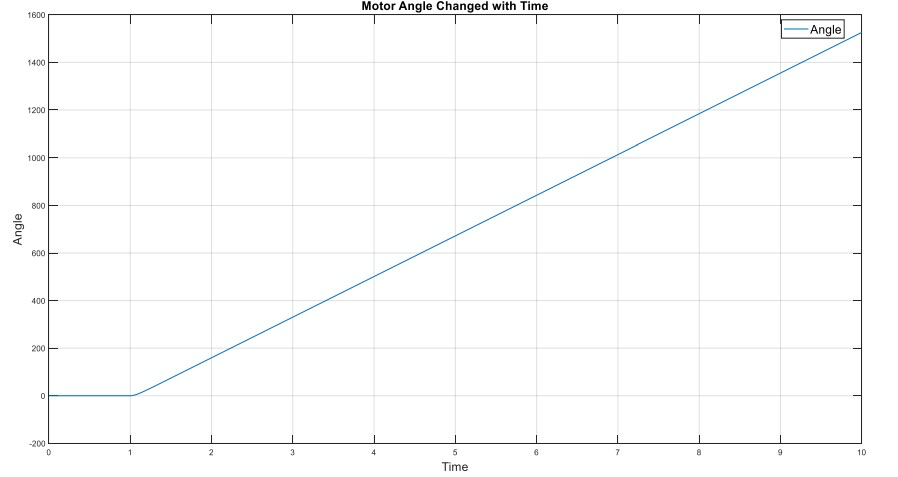
\includegraphics[width=0.7\columnwidth]{imgs/io/e.jpg}
    \caption[Motor angle-time graph]{Motor angle-time graph}
    \label{fig-magnitude}
\end{figure}%

The speed-time graph of the load is as follows
\begin{figure}[H]
    \centering
    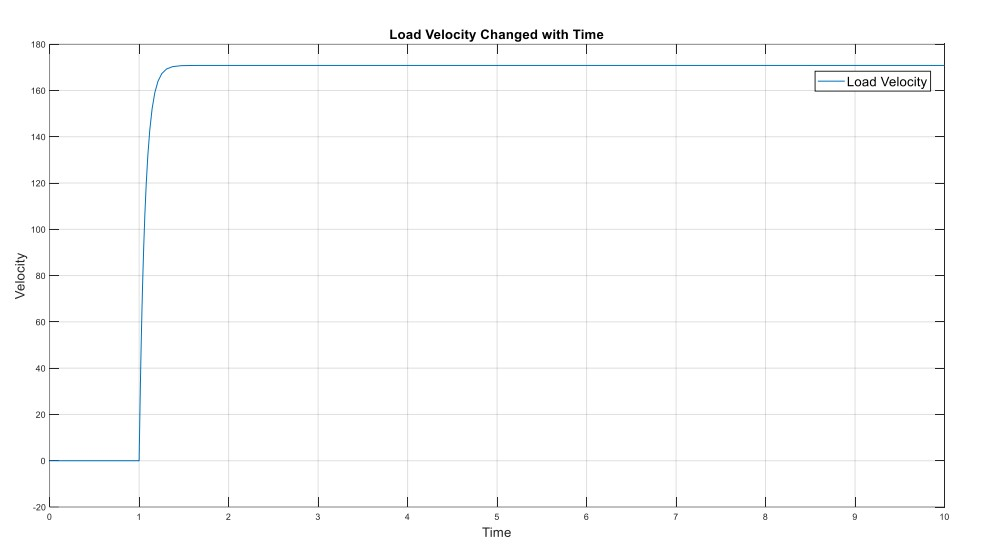
\includegraphics[width=0.7\columnwidth]{imgs/io/f.jpg}
    \caption[load speed-time graph]{load speed-time graph}
    \label{fig-magnitude}
\end{figure}%

The angular position-time graph of the load is as follows.
\begin{figure}[H]
    \centering
    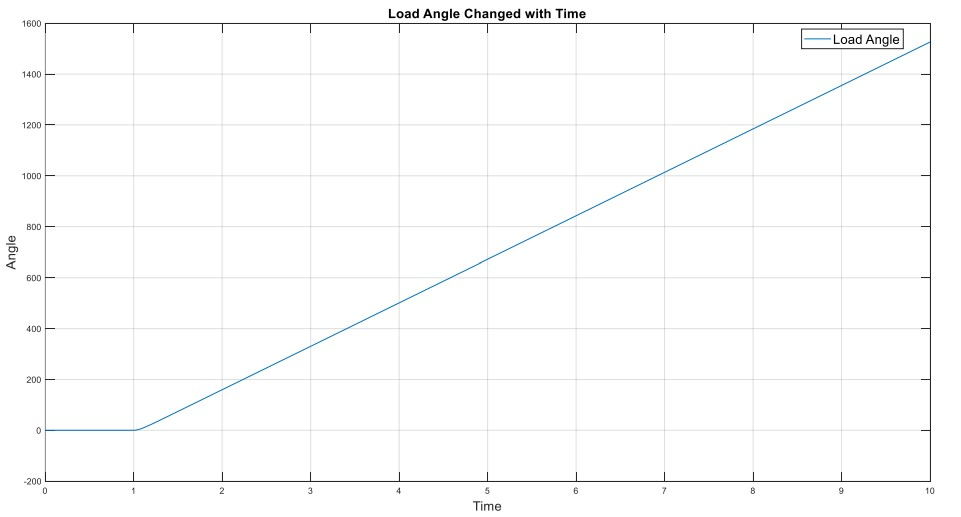
\includegraphics[width=0.7\columnwidth]{imgs/io/g.jpg}
    \caption[load angular position-time graph]{load angular position-time graph}
    \label{fig-magnitude}
\end{figure}%

In the simulation, the voltage of the DC motor was initially given as 5 with a step. Then, with
the effect of back emf, resistance and coil, this voltage was equalized to zero.

\begin{equation}
V = V_{in} - V_{backemf} - RI 
\end{equation}

\begin{figure}[H]
    \centering
    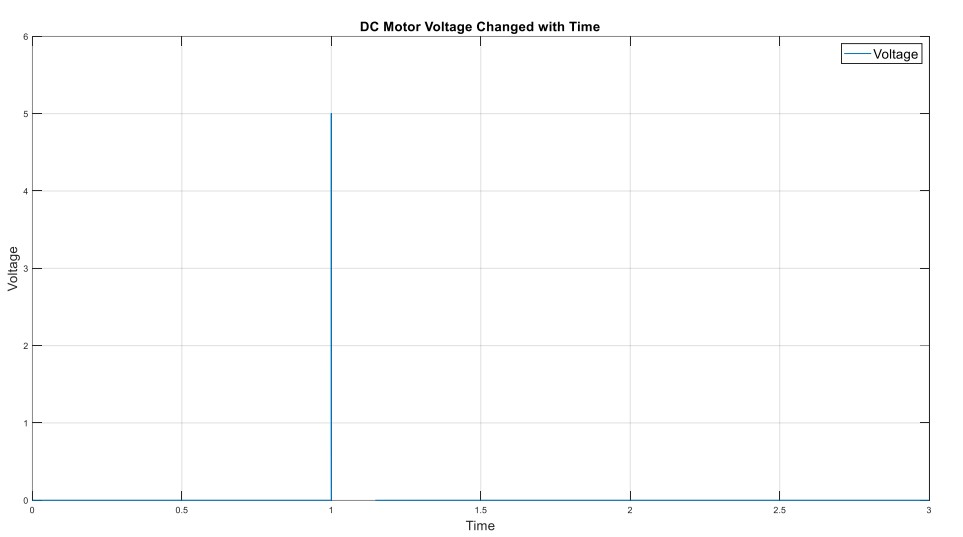
\includegraphics[width=0.7\columnwidth]{imgs/io/h.jpg}
    \caption[DC motor voltage-time graph]{DC motor voltage-time graph}
    \label{fig-magnitude}
\end{figure}%

Motor power is formulated as the product of input voltage and current. Motor power time graph
is as follows

\begin{equation}
P_{DC} = V_{in} I    
\end{equation}

\begin{figure}[H]
    \centering
    \includegraphics[width=0.7\columnwidth]{imgs/io/ı.jpg}
    \caption[Motor power-time graph]{Motor power-time graph}
    \label{fig-magnitude}
\end{figure}%

Output power is equal to the product of the system torque and the motor speed. It is an important
parameter in calculating efficiency. The graph is as follows.

\begin{equation}
P_{out} = \tau W
\end{equation}

\begin{figure}[H]
    \centering
    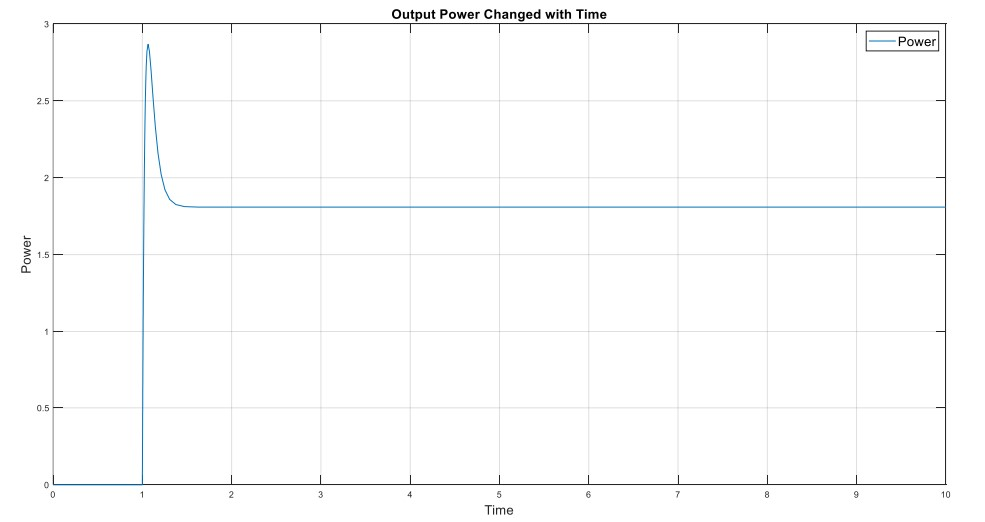
\includegraphics[width=0.7\columnwidth]{imgs/io/i.jpg}
    \caption[Output power-time graph]{Output power-time graph}
    \label{fig-magnitude}
\end{figure}%

In physics, the energy consumed is calculated as the integral of the power. Here, the integral of
the motor power represents the energy consumption of the system

\begin{equation}
Consumption = \int_0^t P_{out} \, dt 
\end{equation}

\begin{figure}[H]
    \centering
    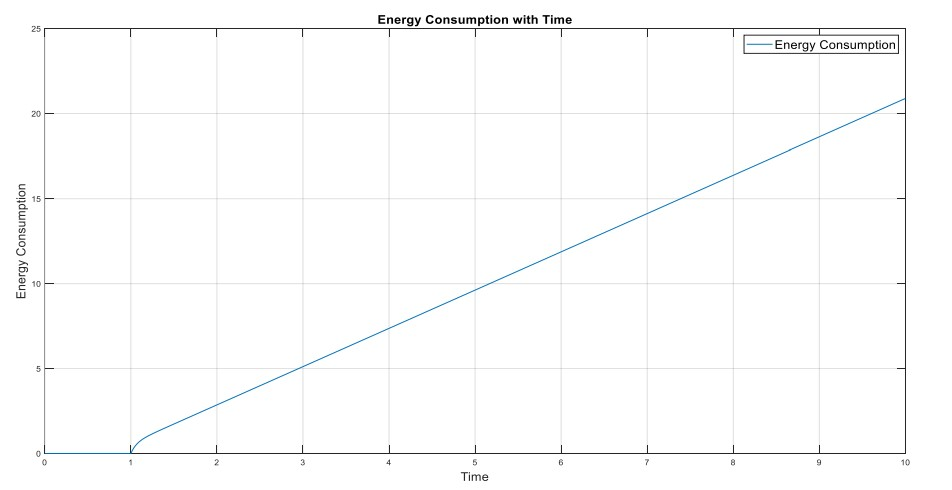
\includegraphics[width=0.7\columnwidth]{imgs/io/j.jpg}
    \caption[Energy consumtion-time graph]{Energy consumtion-time graph}
    \label{fig-magnitude}
\end{figure}%

Efficiency is the measure of the extent to which the power given at the input of a system can be
preserved at the output. Because the integral of the power gives the speed. Here, efficiency is
the ratio of the output power to the input power. A gain block was multiplied to calculate as a
percentage. It was determined that our engine operated at 80% efficiency under these
parameters and this load.

\begin{equation}
\eta = \frac{P_{out}}{P_{DC}} 100    
\end{equation}

\begin{figure}[H]
    \centering
    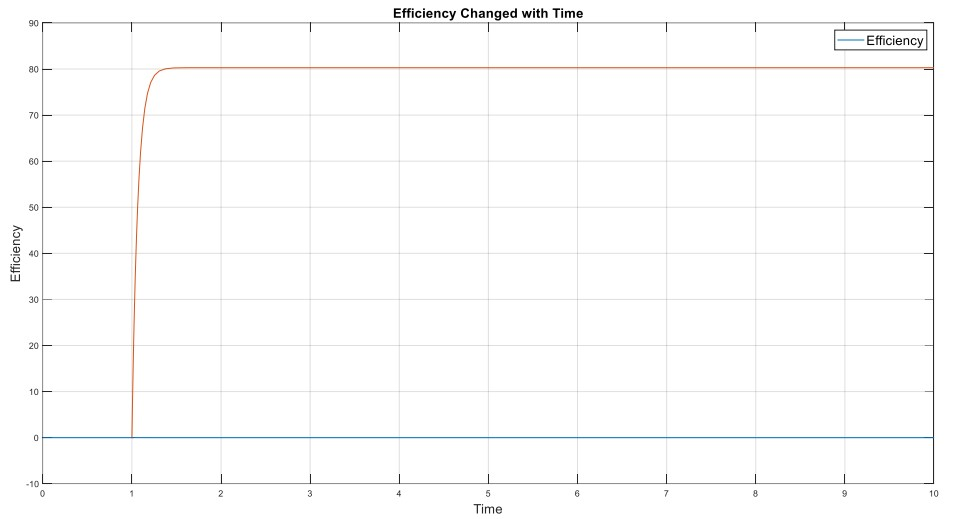
\includegraphics[width=0.7\columnwidth]{imgs/io/k.jpg}
    \caption[Efficiency-time graph]{Efficiency-time graph}
    \label{fig-magnitude}
\end{figure}%





